\documentclass{article}
\usepackage[italian]{babel}
\usepackage[T1]{fontenc}
\usepackage{amsmath,amssymb,amsthm}
\usepackage{enumerate}

\usepackage{epigraph}
\renewcommand{\epigraphrule}{0pt}
\renewcommand{\textflush}{flushepinormal}
\setlength{\epigraphwidth}{0.275\textwidth}
\renewenvironment{flushepinormal}{}{\vspace*{-\baselineskip}}

\usepackage{fontspec}
\usepackage{graphicx}
\usepackage{hyperref}
\usepackage{verbatim}

\graphicspath{ {./images/} }

\title{
  {
    \fontspec[ Path = fonts/ ]{Symbola}
    \symbol{"1F17C}\symbol{"1F435}\symbol{"1F17D}\symbol{"1F17A}ey
  } \large \\
  \small Relazione del progetto per l'insegnamento di Algoritmi e strutture di
  dati
}

\author{
  Gaia Clerici (\#971338),
  Stefano Volpe (\#969766)
}

\date{
	Universit\`a di Bologna \\
  \today
}

\begin{document}

\maketitle
\thispagestyle{empty}

\begin{figure}[h]
  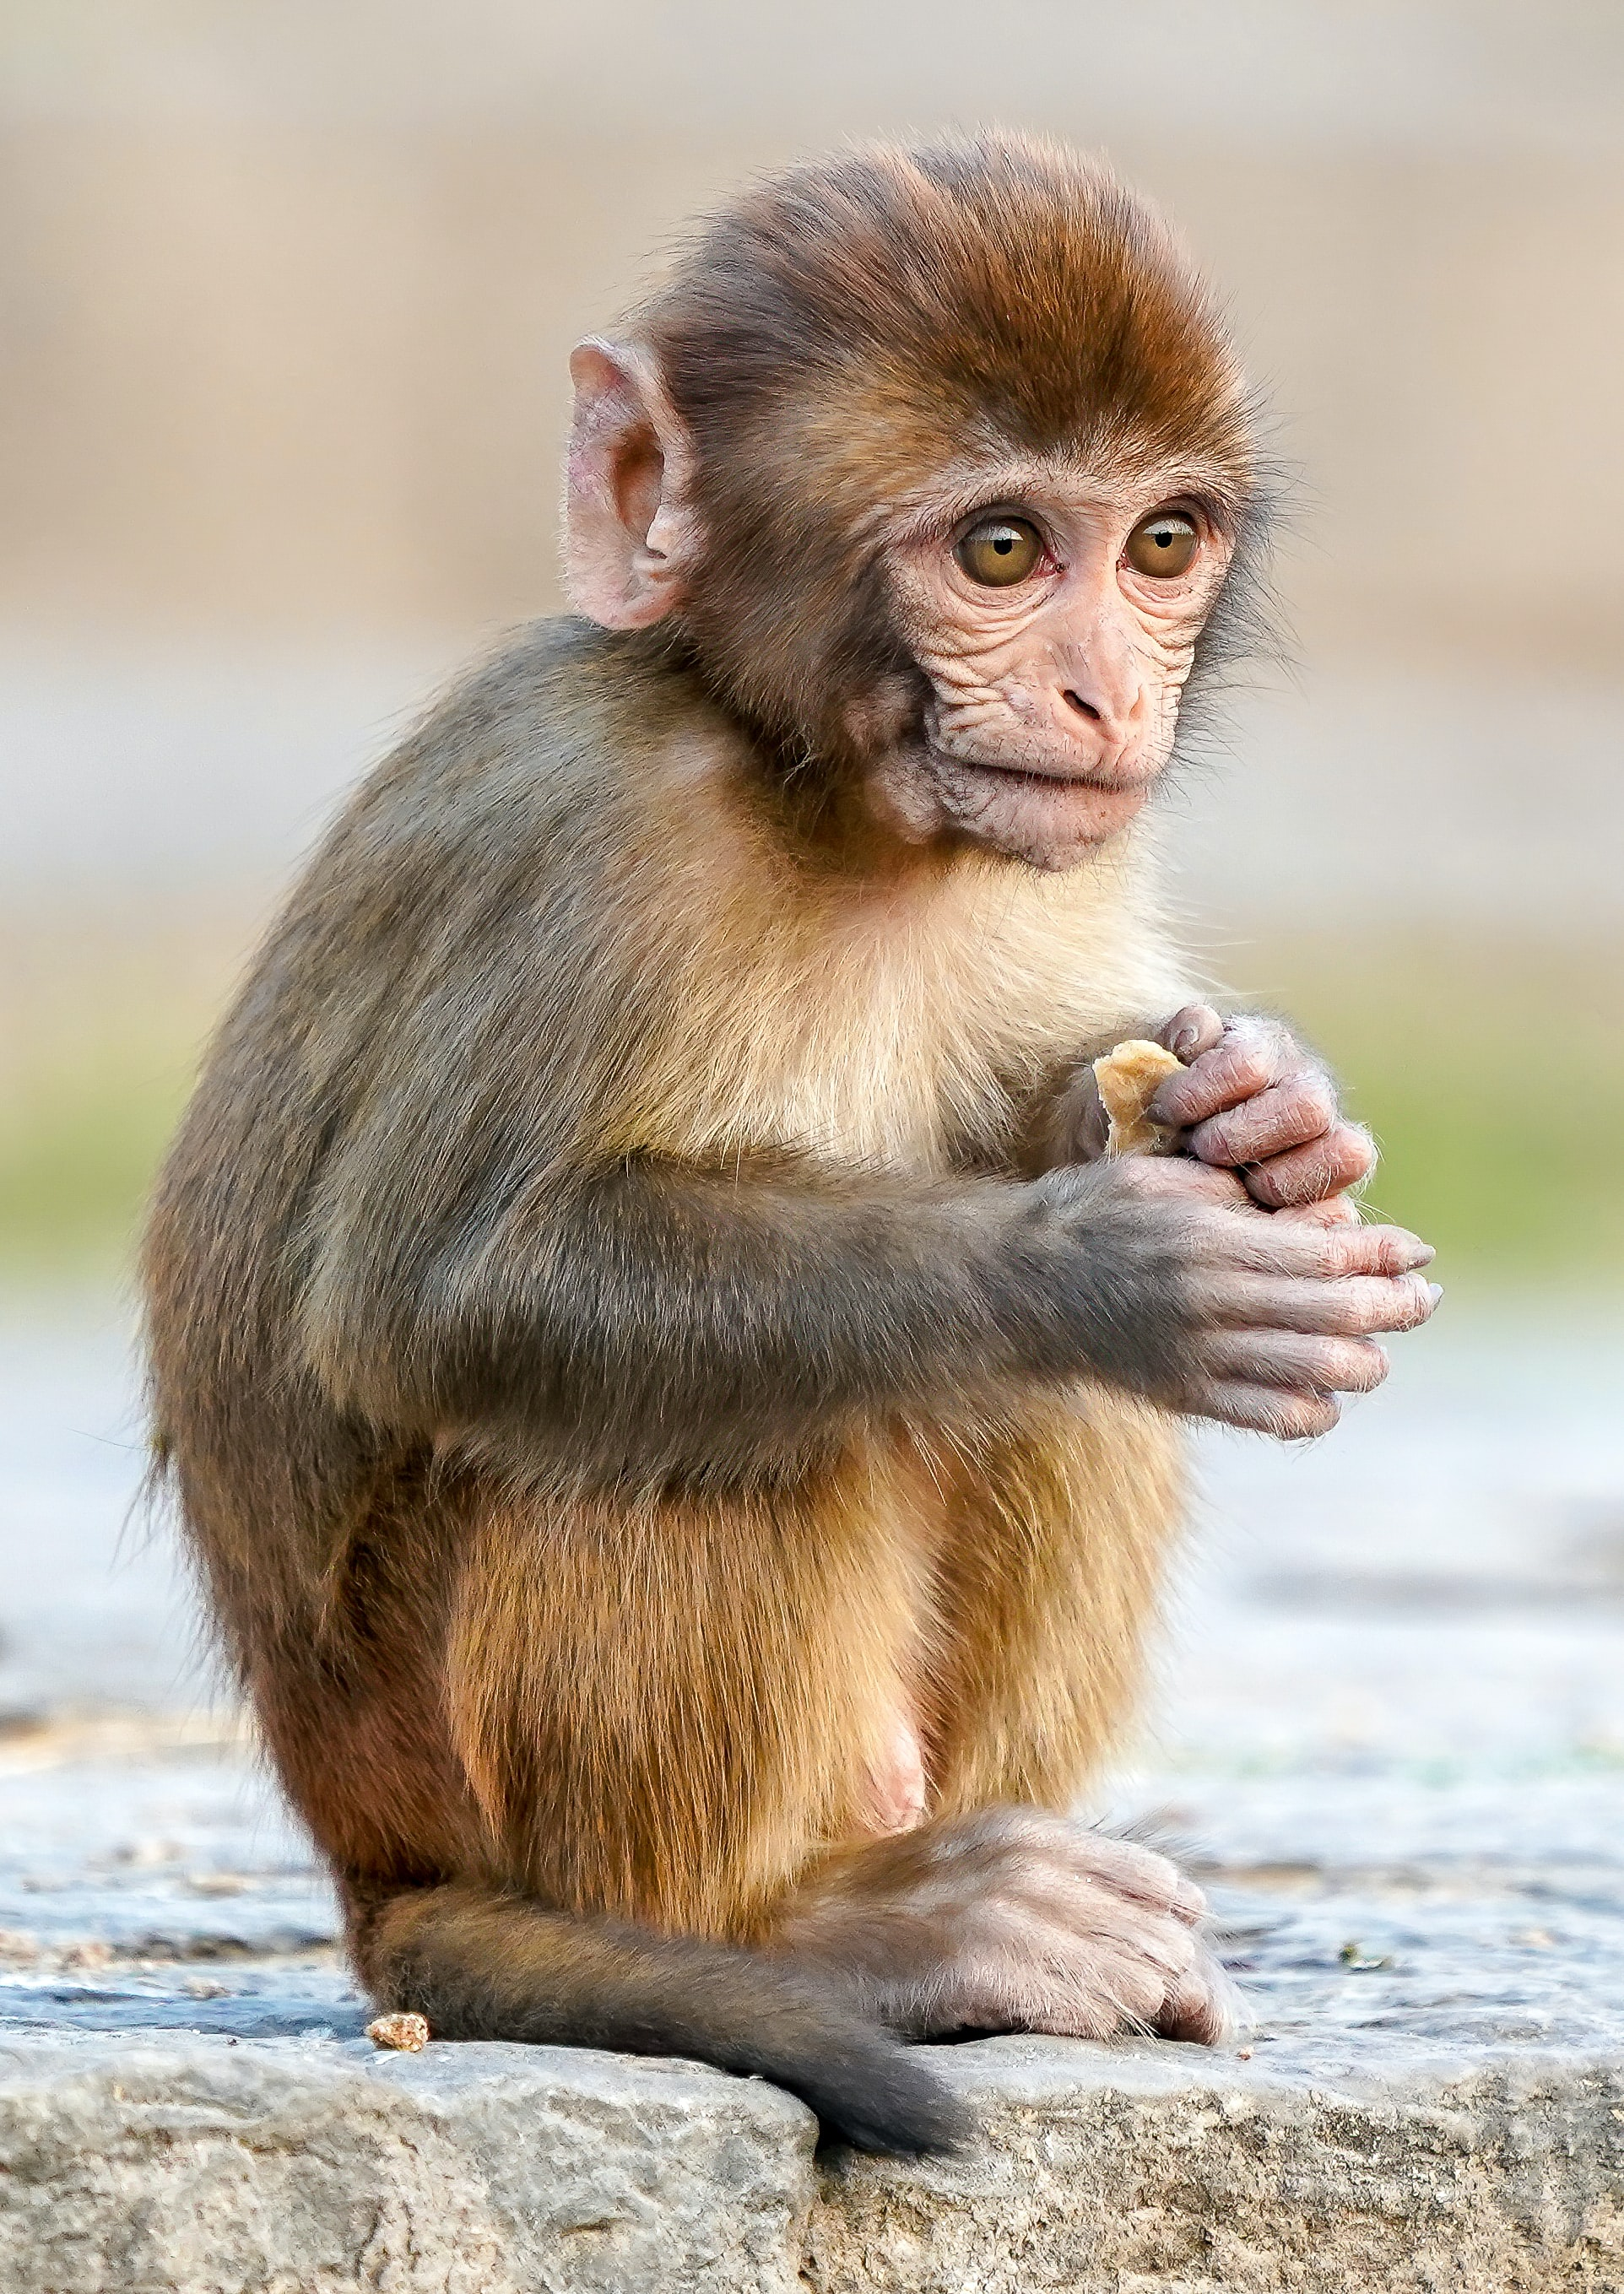
\includegraphics[width=0.75\textwidth]{monkey}
  \centering
  \caption{\href{https://unsplash.com/photos/daC7ji1EMHM}{una scimmia
  (foto di Bob Brewer)}}
\end{figure}

\pagebreak

\epigraph{Fa' la brava scimmietta.}{\textit{L'uomo con il cappello giallo}}

\tableofcontents

\section{Specifiche}

\subsection{Il gioco: \emph{m,n,k-game}}

Il gioco \emph{m,n,k-game} è deterministico, a turni, a due giocatori, a somma
zero e con informazione perfetta. In una partita, i due agenti si alternano nel
marcare una cella vuota in una griglia di dimensione \emph{m}\texttimes \emph{n}
con un simbolo del proprio colore. Se un giocatore allinea in orizzontale,
verticale o diagonale almeno \emph{k} simboli, questi vince la partita e il suo
avversario la perde. Se non rimangono più celle vuote sulla griglia, la partita
finisce in pareggio.

\subsection{Il torneo: la classifica dei giocatori}

Ogni volta che, all'interno del torneo, un giocatore conclude una partita, egli
guadagna: 
\begin{itemize}
  \item 3 punti in caso di una vittoria come secondo giocatore, ma non a
    tavolino;
  \item 2 punti in caso di una vittoria come primo giocatore o a tavolino;
  \item 1 punto in caso di un pareggio;
  \item 0 punti in caso di una sconfitta.
\end{itemize}

\noindent
Le regole del torneo considerano una vittoria "a tavolino" quando l'avversario
non restituisce una mossa entro il tempo limite (approssimativo) di 10 secondi,
o comunque un mossa illegale (già occupata o esterna alla griglia).
Per ognuna delle seguenti configurazioni, ciascun giocatore gioca
esattamente quattro partite contro ogni altro partecipante, di cui due come
primo giocatore e due come secondo giocatore.

\begin{table}[h!]
\centering
\begin{tabular}{ | c | c | c | }
  \hline
  M & N & K \\
  \hline
  3 & 3 & 3 \\
  \hline
  4 & 3 & 3 \\
  \hline
  4 & 4 & 3 \\
  \hline
  4 & 4 & 4 \\
  \hline
  5 & 4 & 4 \\
  \hline
  5 & 5 & 4 \\
  \hline
  5 & 5 & 5 \\
  \hline
  6 & 4 & 4 \\
  \hline
  6 & 5 & 4 \\
  \hline
  6 & 6 & 4 \\
  \hline
  6 & 6 & 5 \\
  \hline
  6 & 6 & 6 \\
  \hline
  7 & 4 & 4 \\
  \hline
  7 & 5 & 4 \\
  \hline
  7 & 6 & 4 \\
  \hline
  7 & 7 & 4 \\
  \hline
  7 & 5 & 5 \\
  \hline
  7 & 6 & 5 \\
  \hline
  7 & 7 & 5 \\
  \hline
  7 & 7 & 6 \\
  \hline
  7 & 7 & 7 \\
  \hline
  8 & 8 & 4 \\
  \hline
  10 & 10 & 5 \\
  \hline
  50 & 50 & 10 \\
  \hline
  70 & 70 & 10 \\
  \hline
\end{tabular}
  \caption{configurazioni previste dal torneo.}
  \label{table:1}
\end{table}

\subsection{L'obiettivo: il giocatore}

Lo scopo del progetto è lo sviluppo di una intelligenza arttficiale per il
giocatore di \emph{m,n,k-game}. Se qualità della risposta e costo temporale
sono prioritari, lo stesso non vale per il costo in memoria: devono comunque
essere evitati sprechi.

\subsection{L'interfaccia: \texttt{mnkgame.MNKPlayer}}

L'interfaccia che l'intelligenza artificiale deve implementare è contenuta nel
pacchetto \verb!mnkgame!. Oltre a un metodo per la selezione della mossa
desiderata, ne viene concesso un altro invocato in fase di inizializzazione
prima di ogni partita.

\section{Analisi del problema}

\subsection{Il valore di gioco teorico}

Per alcune configurazioni, il valore di gioco teorico è già stato dimostrato.
Herik, Uiterwijk e Rijswijck hanno raccolto tali risultati della letteratura
precedente nella seguente tabella.

\begin{table}[h!]
  \centering
  \begin{tabular}{ | c | c | c | }
    \hline
    mnk-game (k=1,2) & Vittoria per il primo giocatore \\
    \hline
    333-game (Tris) & Pareggio \\
    \hline
    mn3-game (m \geq 4,n \geq 3) & Vittoria per il primo giocatore \\
    \hline
    m44-game (m \leq 8) & Pareggio \\
    \hline
    mn4-game (m \leq 5,n \leq 5) & Pareggio \\
    \hline
    mn4-game (m \geq 6,n \geq 5) & Vittoria per il primo giocatore \\
    \hline
    mn5-game (m \leq 6,n \leq 6) & Pareggio \\
    \hline
    15,15,5-game (Go-Moku) & Vittoria per il primo giocatore \\
    \hline
    mnk-game (k \geq 8) & Pareggio \\
    \hline
  \end{tabular}
    \caption{valori di gioco di \emph{m,n,k-game}}
    \label{table:2}
  \end{table}

Tramite l'argomento del "furto di strategia", usato per la prima volta da John
Nash nel 1949, si dimostra che nessuno dei valori di gioco teorico non ancora
aggiunto alla tabella è una vittoria per il secondo giocatore.

\subsection{L'albero di gioco}

Herik, Uiterwijk e Rijswijck classificano \emph{m,n,k-game} come di "categoria
3", ovvero con un'alta complessità dello spazio degli stati e una bassa
complessità dell'albero di gioco. Per poter quantificare meglio il numero di
stati effettivamente appartenenti al nostro albero di gioco, faremo uso del
numero di celle della griglia come indice della dimensione dell'istanza del
problema. Esso vale:

\begin{center}
  $s = m \times n$
\end{center}

Cominciamo osservando che il numero di figli \emph{f} di un qualsiasi nodo non
terminale a profondità \emph{p} coincide con il numero di celle rimaste vuote,
e cioè:

\begin{center}
  $f = s - p$
\end{center}




\section{Strumenti}

\section{Scelte progettuali}

\section{Conclusioni}

\section{Ricerche future}

\section{Bibliografia}

\end{document}
